\section{Theorie}
\label{sec:Theorie}
Ein Fadenpendel der Länge $l$ schwinge im Gravitationspotential der Erde. \\ 

Mit $\vec{r} = \left(\begin{array}{c} l \cos(\phi) \\ l \sin(\phi) \end{array} \right)$ und $\dot{\vec{r}} =\left(\begin{array}{c} -l \sin(\phi) \\ l \cos(\phi) \end{array} \right)$ \\

folgt aus der kinetischen Energie $T = \dfrac{m}{2} v^2 = \dfrac{m}{2} \dot{r}^2$, \\
der potentiellen Energie $V = mgy = mg\sin(\phi)$ und der Lagrange-Funktion $\mathscr{L} = T - V$ mit den Euler-Lagrange-Gleichungen die Bewegungsgleichung \\

$\ddot{\phi} = \dfrac{g}{l}\sin{\phi}$. \\

Die Kleinwinkelnäherung $\sin{\phi} \approx \phi$, die für Winkel $\phi \leq 10°$ gültig ist \cite{wiki:xxx}, liefert die DGL $\ddot{\phi} = \dfrac{g}{l}\phi$ mit der Lösung \\ 
$\phi(t) = C_1 \cos(\omega_0t) + C_2 \sin(\omega_0t)$ , $\omega_0=\sqrt{\dfrac{g}{l}}$. \\

Werden zwei Fadenpendel mit einer Feder aneinander gekoppelt, schwingen sie nicht länger unabhängig voneinander, es stellt sich ein zusätzliches Drehmoment ein. \\

Dabei ist $M_1=D_F(\phi_2-\phi_1)$ und $M_2=D_F(\phi_1-\phi_2)$. \\

Unter diesen Drehmomenten ergibt sich mit dem Trägheitsmoment $J=mL^2$ der Pendel ein System gekoppelter Differentialgleichungen. Es gilt\\

$J\ddot{\phi_1} + D\phi_1 = M_1$ \\

$J\ddot{\phi_2} + D\phi_2 = M_2$. \\

So stellen sich je nach Anfangsbedingung unterschiedliche Schwingmoden ein. Dabei werden gleichsinnige, gegensinnige und gekoppelte Schwingungen unterschieden. \\

\newpage

Für \textbf{gleichphasige Schwingungen}, sprich $\phi_1=\phi_2$, stellt sich für zwei identische Pendel die bereits aus der Schwingung einzelner Pendel bekannte Frequenz \\ 
\begin{equation}
    \omega = \omega_+ = \frac{2π}{T_+} = \sqrt{\frac{g}{l}} \label{eq:omega+}
\end{equation}
mit der Periodendauer 
\begin{equation}
T_+ = 2\pi \omega_+ = 2\pi \sqrt{\dfrac{l}{g}}\,.
\label{eq:T_+}
\end{equation}
ein. Eine solche gleichphasige Schwingung ist in \autoref{fig:gleiSchwi} dargestellt.

\begin{figure}
    \centering
    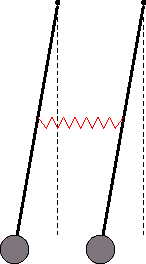
\includegraphics{v106_abb1.pdf}
    \caption{Gleichphasige Schwingung \cite{ap01}.}
    \label{fig:gleiSchwi}
\end{figure}

Bei entgegengesetzten Anfangsauslenkungen ($\phi_1=-\phi_2$) spricht man von einer \\ 
\textbf{gegenphasigen Schwingung}, wie in \autoref{fig:gegSchwi} dargestellt. Die Schwingfrequenz $\omega_-$ ergibt sich dann zu
\begin{equation}
    \omega_- = \frac{2π}{T_-} = \sqrt{\frac{g+2K}{l}} \label{eq:omega-}
\end{equation}
wobei $K$ als Kopplungskonstante der Feder definiert wird.
Die Periodendauer ist dann 
\begin{equation}
    T_- = 2 \pi \omega_- = 2 \pi \sqrt{\dfrac{l}{g+2K}} \,.
\label{eq:T_-}
\end{equation}

\begin{figure}
    \centering
    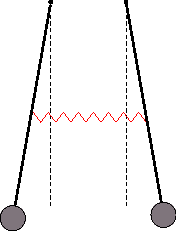
\includegraphics{v106_abb2.pdf}
    \caption{Gegenphasige Schwingung \cite{ap01}.}
    \label{fig:gegSchwi}
\end{figure}

\newpage

\textbf{Gekoppelte Schwingungen} bezeichnen Schwingungen, bei denen für eine der Anfangsauslenkungen $\phi_n = 0$ gilt.
Das schwingende Pendel beginnt, seine Energie auf das ruhende Pendel zu übertragen, seine Amplitude nimmt also langsam ab, während die des nicht ausgelenkten Pendels immer weiter zunimmt und ihr Maximum erreicht, sobald das andere Pendel ruht.
Dieser Vorgang der Energieübertragung wiederholt sich immer wieder, die Zeit zwischen zwei Ruhezeiten eines Pendels wird dabei als Schwebungsdauer $T_S$ mit der Schwebungsfrequenz $\omega_S$ bezeichnet. \\
Dabei gilt 
\begin{equation}
    \omega_S = \frac{2π}{T_S} =  |\omega_+ - \omega_-| \label{eq:omegaS}
\end{equation}
und
\begin{equation}
    T_S = \dfrac{T_+ T_-}{T_+ - T_-} \label{eq:T_S} \,.
\end{equation}
Die Anfangsauslenkungen einer gekoppelten Schwingung sind in \autoref{fig:gekoSchwi} dargestellt.

\begin{figure}
    \centering
    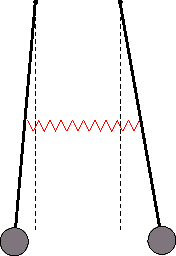
\includegraphics{v106_abb3.pdf}
    \caption{Gekoppelte Schwingung \cite{ap01}.}
    \label{fig:gekoSchwi}
\end{figure}

Der Kopplungsgrad $K$ der beiden Pendel ist dabei definiert als
\begin{equation} 
    K := \dfrac{\omega_-^2-\omega_+^2}{\omega_-^2 + \omega_+^2} = \dfrac{T_+^2 - T_-^2}{T_+^2 + T_-^2} \text{.}
\label{eq:Kopplungsgrad}
\end{equation}

% Fertig und korrigiert



